% !TeX encoding = UTF-8
%



\subsection{Abdeckung}
\label{Abschnitt:Tests:Statistik:Abdeckung}

% Coverage, welche unser lokales Werkzeug ausgibt.
\newcommand\VSLocalCoverage{\textasciitilde~86,20 \%}

% Coverage, welche unser Online-Wekrzeug ausgibt.
\newcommand\OnlineLocalCoverage{\textasciitilde~89,18 \%}

% Coverage im Bezug auf alle vorhandenen Klassen.
\newcommand\VSGlobalCoverage{\textasciitilde~30,00 \%}

Auf den folgenden Seiten steht die Kurzversion des aus den Daten von \hyperref[Abschnitt:Tests:Werkzeuge:Automatisiert:OpenCover]{\mousecursor~OpenCover} generierten Berichts zur Testabdeckung durch Komponententests.
Der prozentuale Anteil bezieht sich hierbei auf die Anzahl der abgedeckten Zeilen Code (LOC), aller als relevant eingestufter Komponenten. In Tabelle \ref{Abschnitt:Tests:Statistik:Abdeckung:Tabelle} sind die Ergebnisse aufgelistet.

\begin{longtable}{p{0.75\hsize}p{0.25\hsize}}

	\caption{Testabdeckung durch Komponententests\\~\\}
	\label{Abschnitt:Tests:Statistik:Abdeckung:Tabelle}
	\\

	  Selektiv (lokal, .NET 4.5.1, XNA 4.0):
	& \VSLocalCoverage \\
	
	  Selektiv (online, Mono 3.2, MonoGame-SDL2):
	& \OnlineLocalCoverage \\
	
	  Gesamt:
	& \VSGlobalCoverage \\

\end{longtable}

~\\

Die selektive Testabdeckung bezieht sich auf den Anteil aller Klassen, die wir nicht herausgefiltert haben.
Dabei verwendeten wir ein lokales- und ein Online-Werkzeug, die beide auf OpenCover basieren.
~\\

Online läuft die aktuellste Version von OpenCover unter Ubuntu 14.04 mit Mono 3.2, lokal läuft OpenCover unter .NET 4.5.1.
Lokal erreichen wir eine Abdeckung von \VSLocalCoverage~und online \OnlineLocalCoverage.
~\\

Der Unterschied kommt hauptsächlich durch die unterschiedlichen Compiler und Laufzeitumgebungen zustande, da Mono und .NET unterschiedlich effizient in sowohl der
Kompilierung als auch in der Ausführung des Codes sind und jeweils auch im Debug-Modus unterschiedliche Anweisungen wegoptimieren.
~\\

Wir geben hier beide Werte an, da diese für uns auch laufend eine Selbstkontrolle darstellen.
Die Gesamt-Testabdeckung wurde unter Mono ermittelt und ist um einiges niedriger als die selektiven Testabdeckungen.
Dies liegt daran, dass wir alle GUI-Klassen selbst geschrieben haben (Widgets, etc.) und diese größtenteils nicht testen konnten.
Wir verweisen an dieser Stelle nochmals auf die ausführliche Erklärung unter \hyperref[Abschnitt:Tests:Nicht]{\mousecursor~Abschnitt \ref{Abschnitt:Tests:Nicht}, ab S. \pageref{Abschnitt:Tests:Nicht}}.


%\newgeometry{left=8cm,bottom=0.1cm,top=1cm,right=0.1cm}
\newgeometry{includehead,includefoot,
  left=1.in,right=1.0in,
  top=0.6in,bottom=0.8in,
  headheight=20pt,headsep=0.25in,
  footskip=0.3in}

\thispagestyle{empty}
\pagestyle{empty}

\begin{figure}[h!]

	\centering{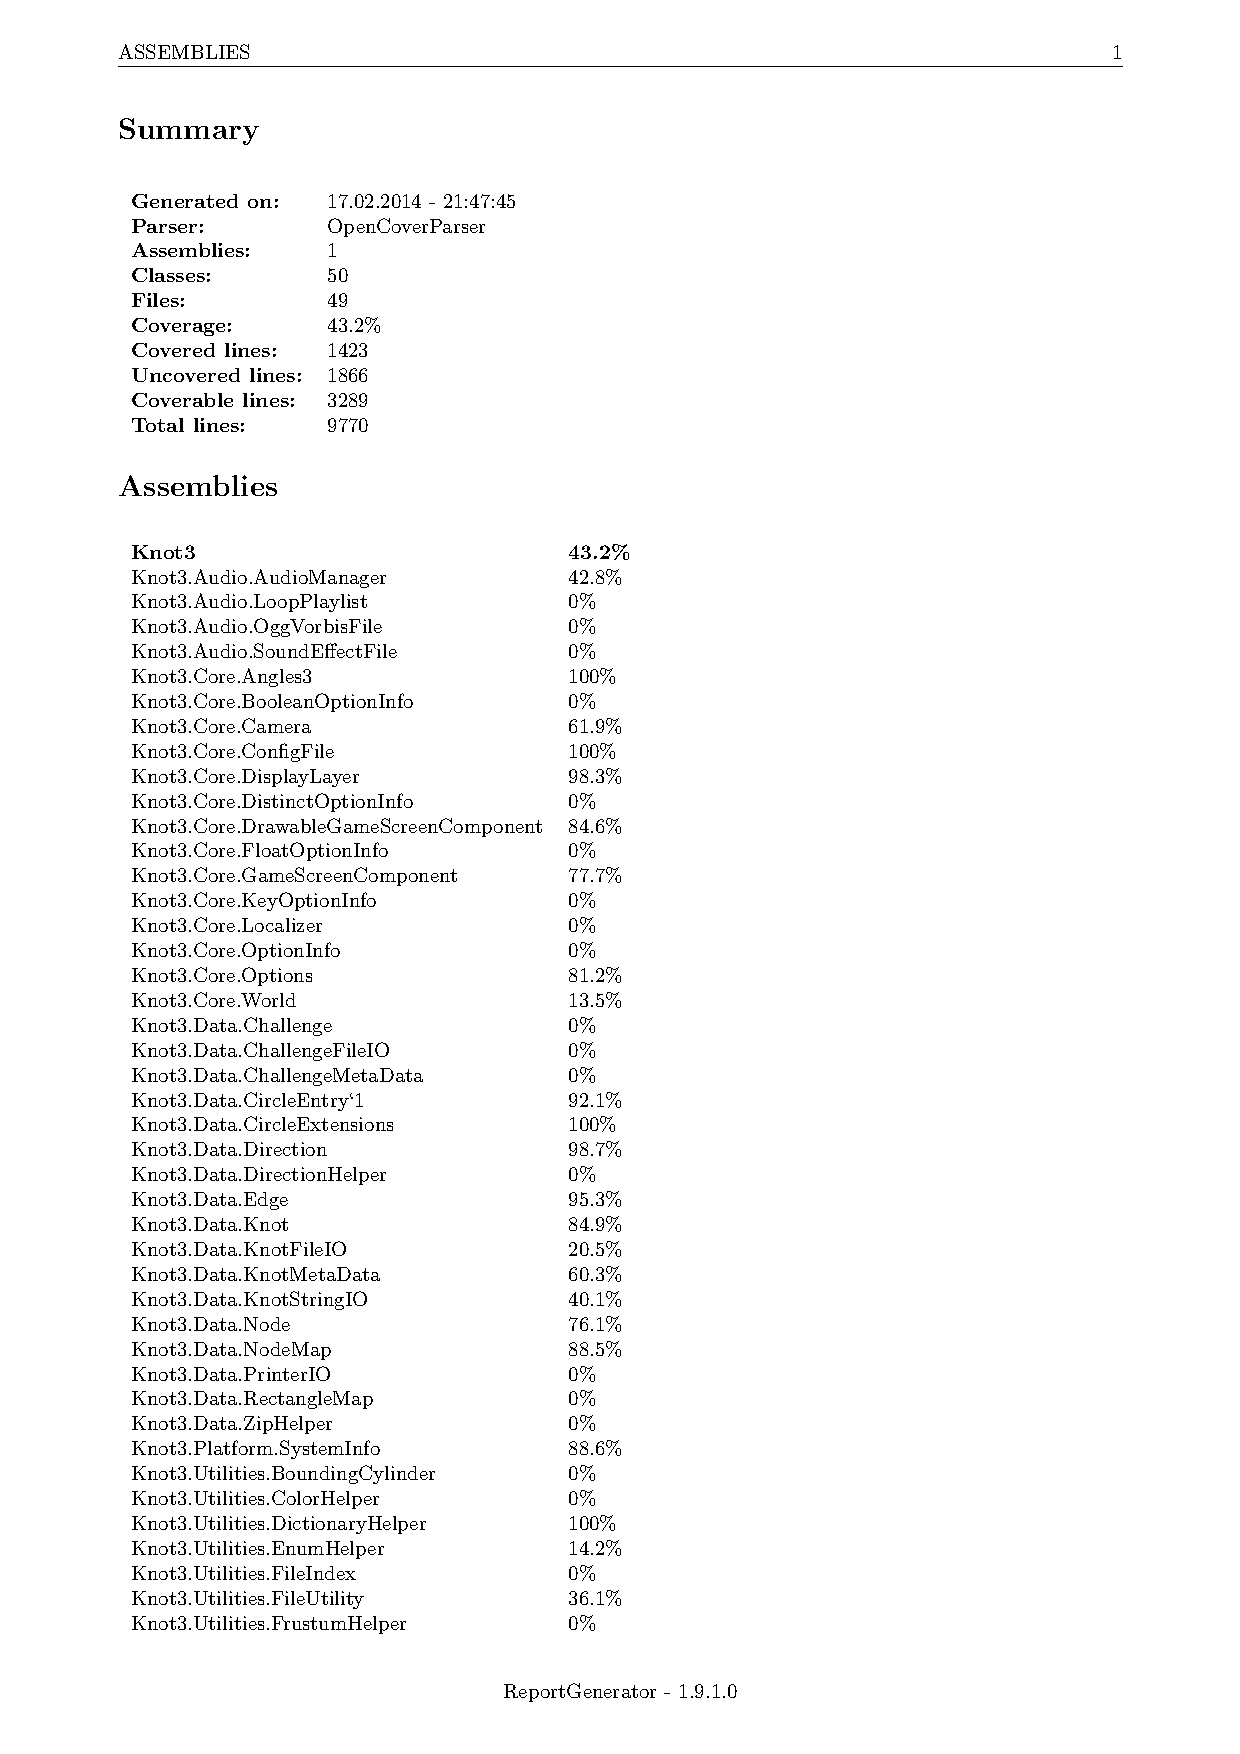
\includegraphics[page=1,scale=1.0]{Inhalt/Tests/Abdeckung/OpenCover_Bericht_uebersicht.pdf}} 
   
\end{figure}


\begin{figure}[h!]

	\centering{\includegraphics[page=2,scale=1.0]{Inhalt/Tests/Abdeckung/OpenCover_Bericht_uebersicht.pdf}} 
   
\end{figure}

\restoregeometry

\thispagestyle{plain}
\pagestyle{plain}
